\chapter{Different control strategies}

\section{Manoeuvring the vessel using the LOS method}
Path-following problems for vessels are often solved by implementing \ac{LOS} algorithms. Opposite to other position control algorithms, where the vessel may be driven both in longitudinal and transversal directions to converge to a path, the \ac{LOS} algorithm gives a more natural motion towards the desired path. This is done by giving a more natural reference to the heading of the vessel. One of the advantages of this is that it can be applied both to fully actuated and under actuated vessels.

Since it is only the leader, and not any of the followers, who need to follow a path, this is only applied on one vessel. This can also be extended to a leader in a virtual structure. To apply the \ac{LOS} algorithm a setup is needed. To get an overview of the functionality of the \ac{LOS} algorithm see figure~\vref{fig:allinallframes}.
\begin{figure}[htbp]
	\centering
	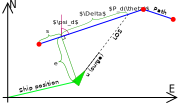
\includegraphics[width=\textwidth]{fig/allinallframes}
	\caption{A vessel placed beside the path and uses the \ac{LOS} algorithm to get back on track.}
	\label{fig:allinallframes}
\end{figure}
On the figure is a green vessel that needs to get onto the blue path. The red point at the path is desired position $\theta$ at time $t$, $\textbf{p}_d(\theta)$. From this point a tangent to the path is made, which crosses the vessels heading. The angle from north to the tangents slope is the \textit{desired heading}, $\psi_d$, for the vessel. This will make it converge to the reference path over time. $s$ along the tangent is the \textit{along track error} and $e$ from the vessel to the path is the \textit{cross track error}, which are  the two that needs to be minimized to make the vessel converge to the path. $\epsilon$ is the position of the vessel relative to the reference point on the path.

\subsubsection{The \ac{LOS} algorithm}
The vessel has a generalized position in the ${n}$-frame given as
\begin{align}
\eta = col(\textbf{p},\psi)\quad , \quad \textbf{p} = col(x,y)
\end{align}
with dynamics given by
\begin{align}
\dot{\eta} = \textbf{R}(\psi)\boldsymbol{\nu}
\end{align}
where $\boldsymbol{\nu} = col(u,v,r)$.\\
The path can be parametrized by a set of points with
\begin{align}
\mathcal{P} = {\textbf{x}}\in\mathds{R}^2 : \quad \exists \theta \in \mathds{R} \quad s.t. \quad \textbf{x} = \textbf{p}_d(\theta)
\end{align}
where $\textbf{p}_d(\theta) := col(x_d(\theta),y_d(\theta))$ is a smooth function. The path needs to be smooth such that the \ac{LOS} algorithm makes the vessel converge to the path. When applying the \ac{LOS} algorithm it makes the setup immune to sideslip error. This is due to the minimization of $s$ and $e$ when the vessel surges towards the path.

For a given value of $\theta$, being a specific point on the path, is the tangent to the path introduced with origin located in $\textbf{p}_d(\theta)$. The orientation of the reference frame, being the desired heading, is given by
\begin{align}
\psi_d(\theta) = \arctan2\left(\frac{y_d^\theta(\theta)}{x_d^\theta(\theta)}\right)
\end{align}
The position of the vessel from the desired position on the path is given in path-tangential coordinates according to
\begin{align}
\epsilon(\textbf{p},\theta) = col(s(\textbf{p},\theta),e(\textbf{p},\theta))
\end{align}
where $s(\textbf{p},\theta)$ is the along track error and $e(\textbf{p},\theta)$ is the cross track error. These are given on figure~\vref{fig:allinallframes}, and is the errors from the vessel to the desired point on the path. This position can also be expressed using the rotation of the $\epsilon$-vector by
\begin{align}
\epsilon(\textbf{p},\theta) = \textbf{R}_{2D}(\psi_d(\theta))^T(\textbf{p}-\textbf{p}_d(\theta))
\end{align}
where
\begin{align}
\textbf{R}_{2D}(\psi_d(\theta)) = 
\begin{bmatrix}
cos(\psi_d(\theta) & -sin(\psi_d(\theta)\\
sin(\psi_d(\theta) & cos(\psi_d(\theta)
\end{bmatrix}
\end{align}